

\subsection{Output Analysis of $S(R)$}


As introduced in Fig.~\ref{fig:pbc_lrws}, periodic boundary conditions
construct the infinite two-dimensional tiling domain by filling all of
$R^2$ by copies of the primitive cell without overlapping or leaving
any gaps. In other words, eight identical obstacles with absorbing
boundary in other copies of the image are neighbouring and impose a
restriction on particles' movement and finally absorb them in LRWs.


In other words, there has an infinite number of obstacles
with absorbing boundary conditions building a confining domain.
          
     \begin{figure}
        \centering
        \begin{subfigure}[b]{0.45\textwidth}
          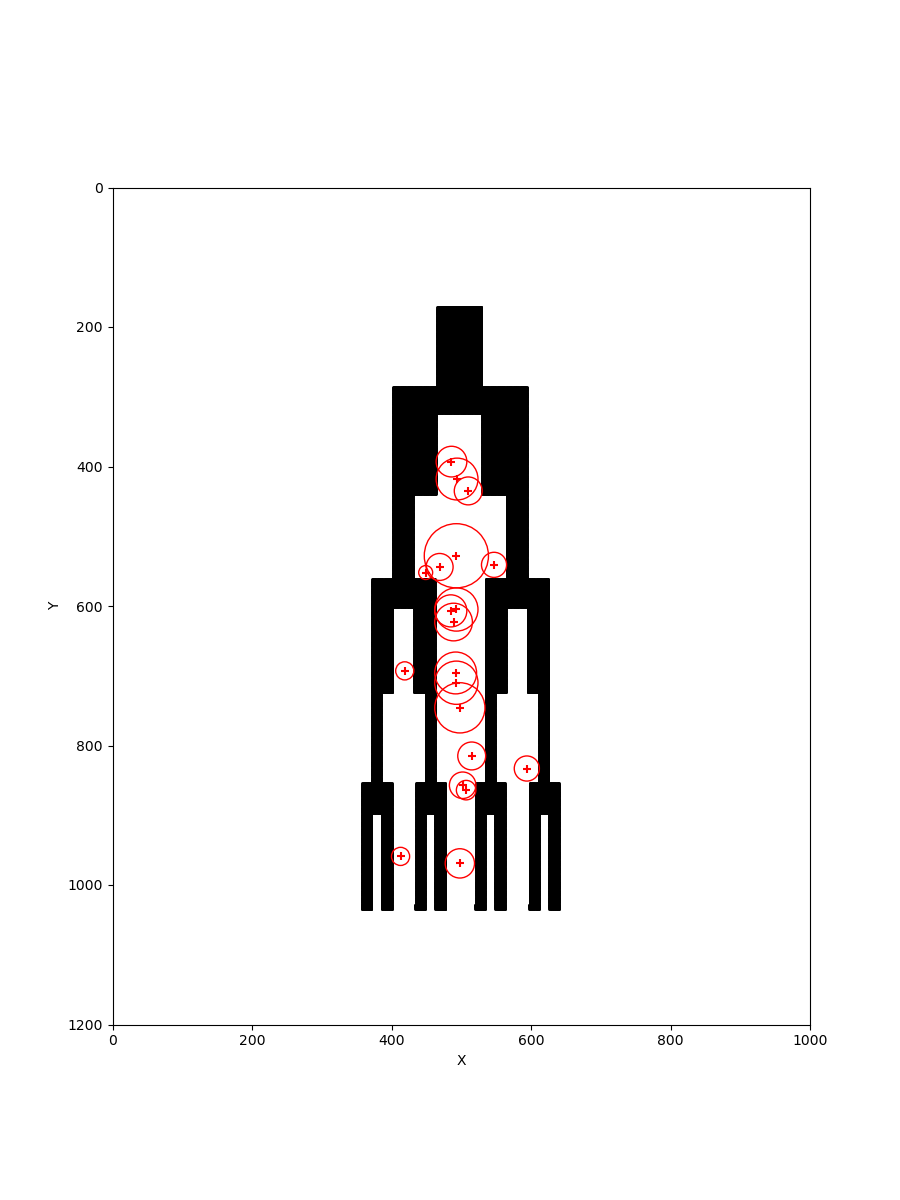
\includegraphics[width=\textwidth]{G_1_L_3_first_circles_red.png}
          \caption{}
          \label{fig:G_1_L_3_first_circles_red}
        \end{subfigure}
        \hfill
        \begin{subfigure}[b]{0.45\textwidth}
          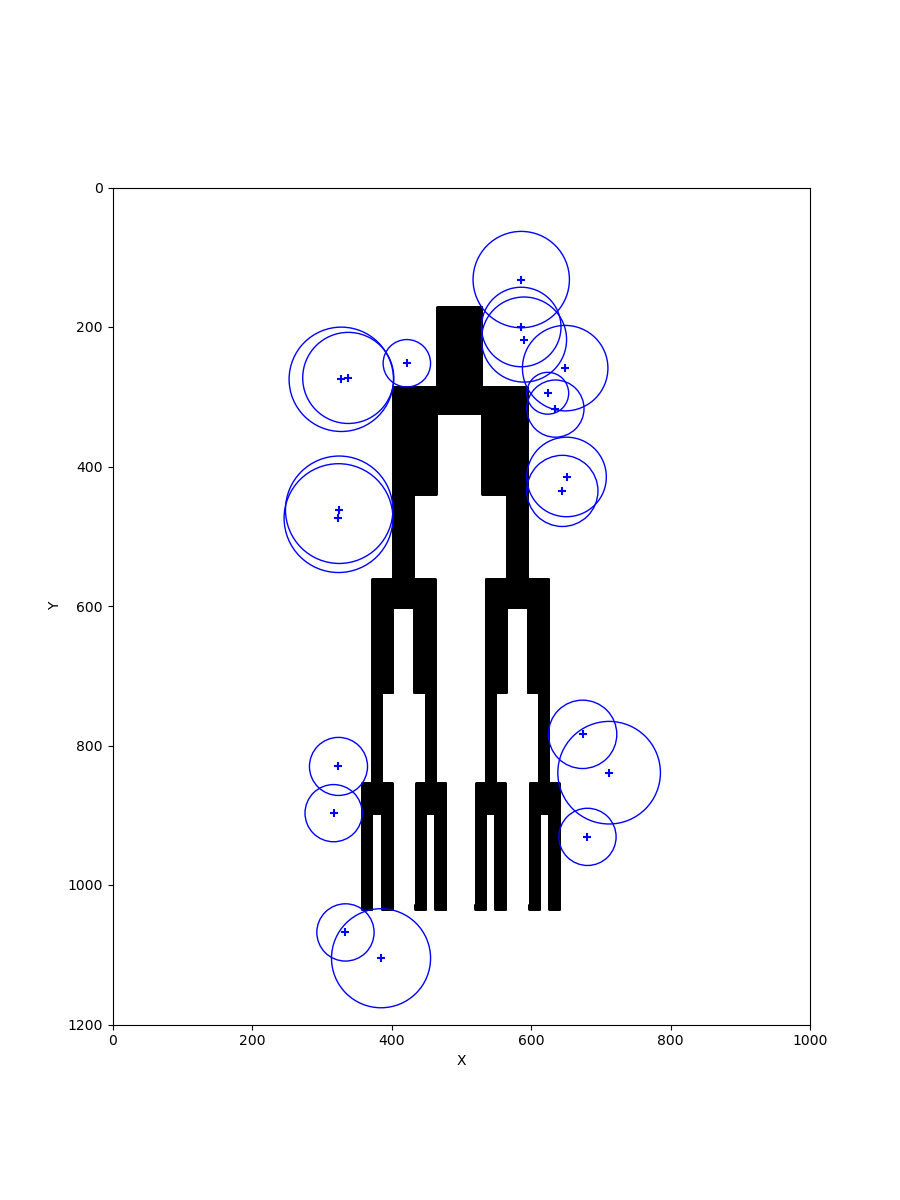
\includegraphics[width=\textwidth]{G_1_L_3_first_circles_blue.png}
          \caption{}
          \label{fig:G_1_L_3_first_circles_blue}
        \end{subfigure}
        \vskip\baselineskip
        \begin{subfigure}[b]{0.45\textwidth}
          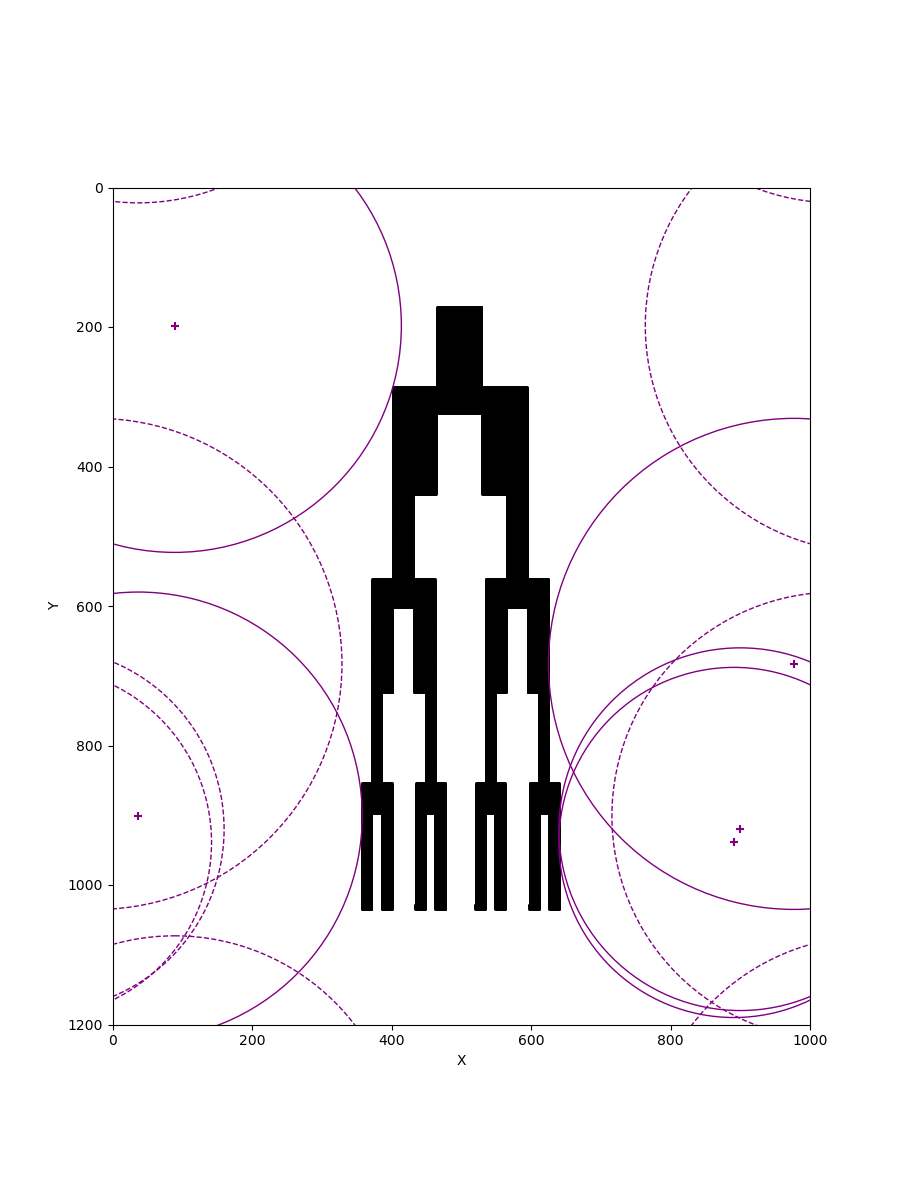
\includegraphics[width=\textwidth]{G_1_L_3_first_circles_purple.png}
          \caption{}
          \label{fig:G_1_L_3_first_circles_purple}
        \end{subfigure}
        \hfill
        \begin{subfigure}[b]{0.45\textwidth}
          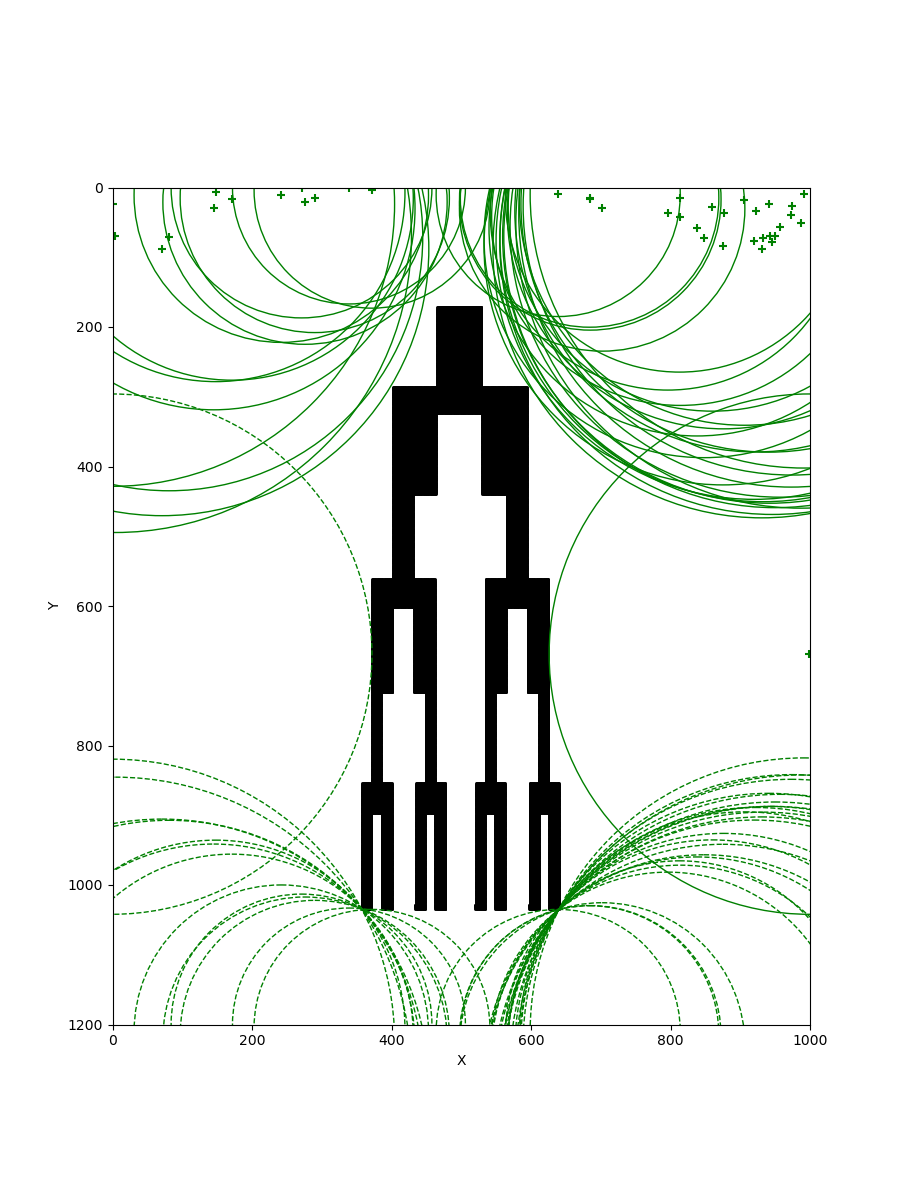
\includegraphics[width=\textwidth]{G_1_L_3_first_circles_green.png}
          \caption{}
          \label{fig:G_1_L_3_first_circles_green}
        \end{subfigure}
        \caption{This figure shows four types of the largest discs
          centred at some colourful plus symbols, $+$, which are
          initial positions of particles in LRWs. The radius of a disk
          is the shortest distance from the initial site to the
          absorbing boundary. As shown in (a) and (b), if particles
          are close to the target object, the completed discs can be
          drawn with the solid line. Specifically, the red discs
          between or inscribed in branches imply the spacing
          information of branching structure. The blue discs closely
          near the target object characterize a portion of empty
          space, where particles can wander around and are nearly
          impossible to escape from the image. As explained in
          Fig.~\ref{fig:pbc_lrws}, periodic boundary conditions can
          eliminate the edge effect and produce an infinite
          system. Suppose the initial locations are slightly far away
          from the branching structures or close to the image edges as
          illustrated in (c) and (d), respectively. Due to periodic
          boundary conditions, the entire circle consists of the solid
          and dashed arc. It indicates that particles will likely pass
          through the image edges and enter the adjacent image
          (i.e. reappear on the other sides of the image). }
        \label{fig:G_1_L_3_first_circles}
     \end{figure}
     

        

        



    \subsubsection{Interpretation of Survival Curves}

     \begin{figure}
        \centering
        \begin{subfigure}[b]{0.45\textwidth}
          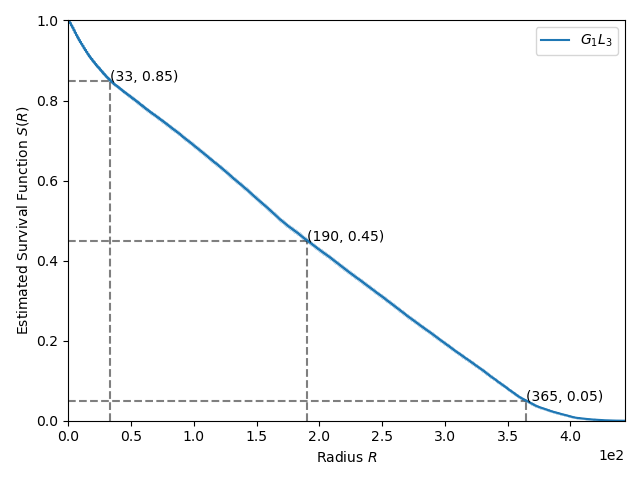
\includegraphics[width=\textwidth]{initial_radius_seg_curve_G_1_L_3.png}
          \caption{}
          \label{fig:G_1_L_3_radius_sf}
        \end{subfigure}
        \hfill
        \begin{subfigure}[b]{0.45\textwidth}
          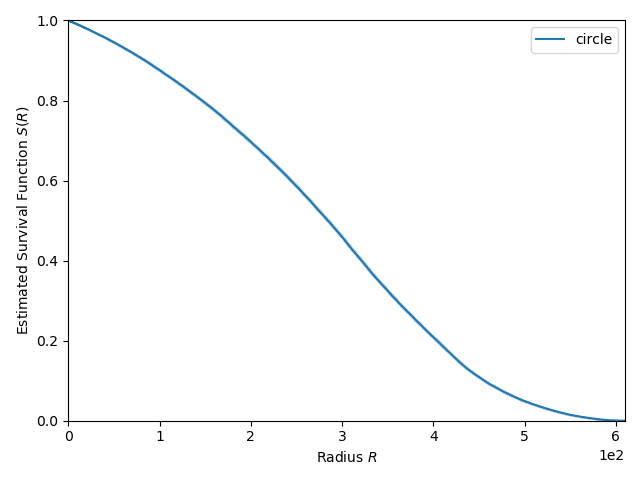
\includegraphics[width=\textwidth]{circle_initial_radius_sf.png}
          \caption{}
          \label{fig:circle_radius_sf}
        \end{subfigure}
        \caption{}
        \label{fig:shape_sf_radius}
     \end{figure}


     \begin{figure}
        \centering
        \begin{subfigure}[b]{0.45\textwidth}
          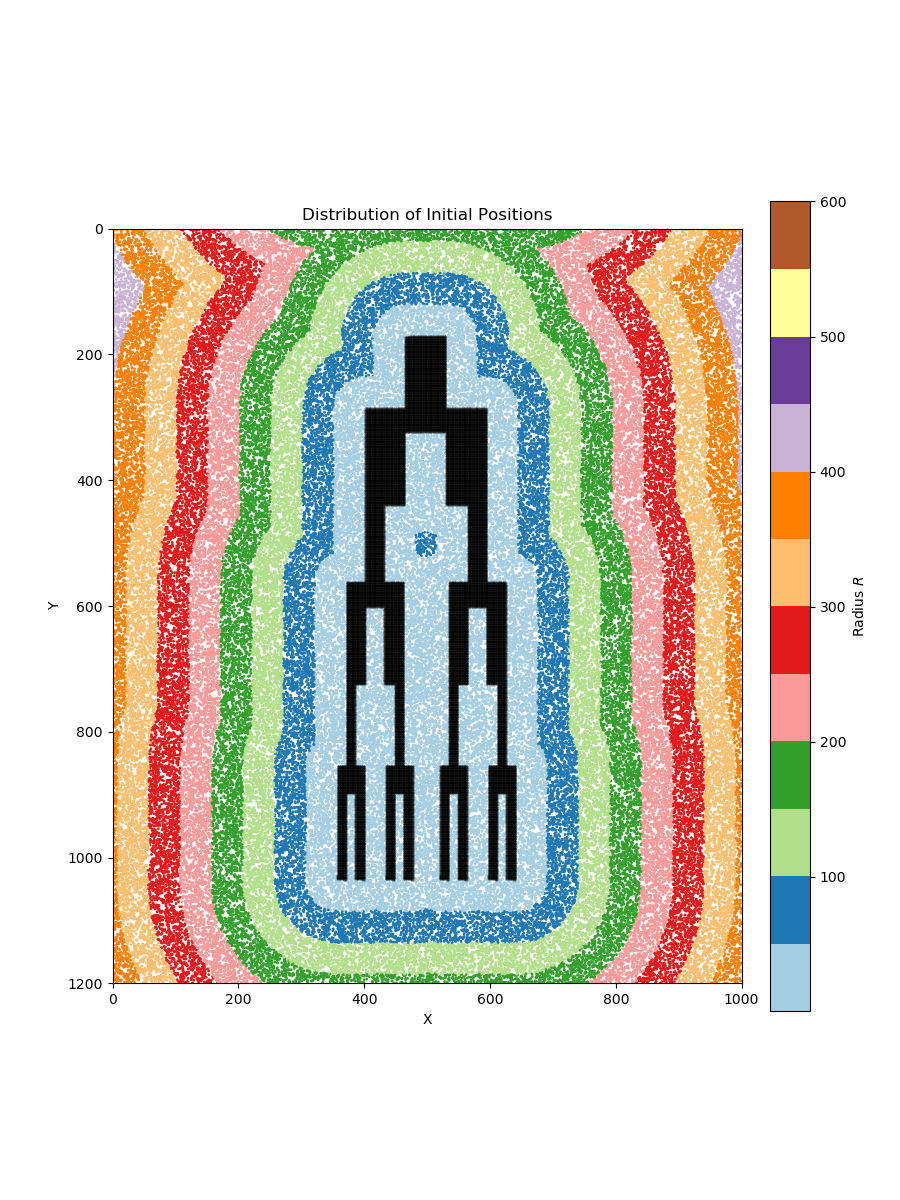
\includegraphics[width=\textwidth]{G_1_L_3_initial_radius_color_initial_pos.png}
          \caption{}
          \label{fig:G_1_L_3_radius_initial_pos}
        \end{subfigure}
        \hfill
        \begin{subfigure}[b]{0.45\textwidth}
          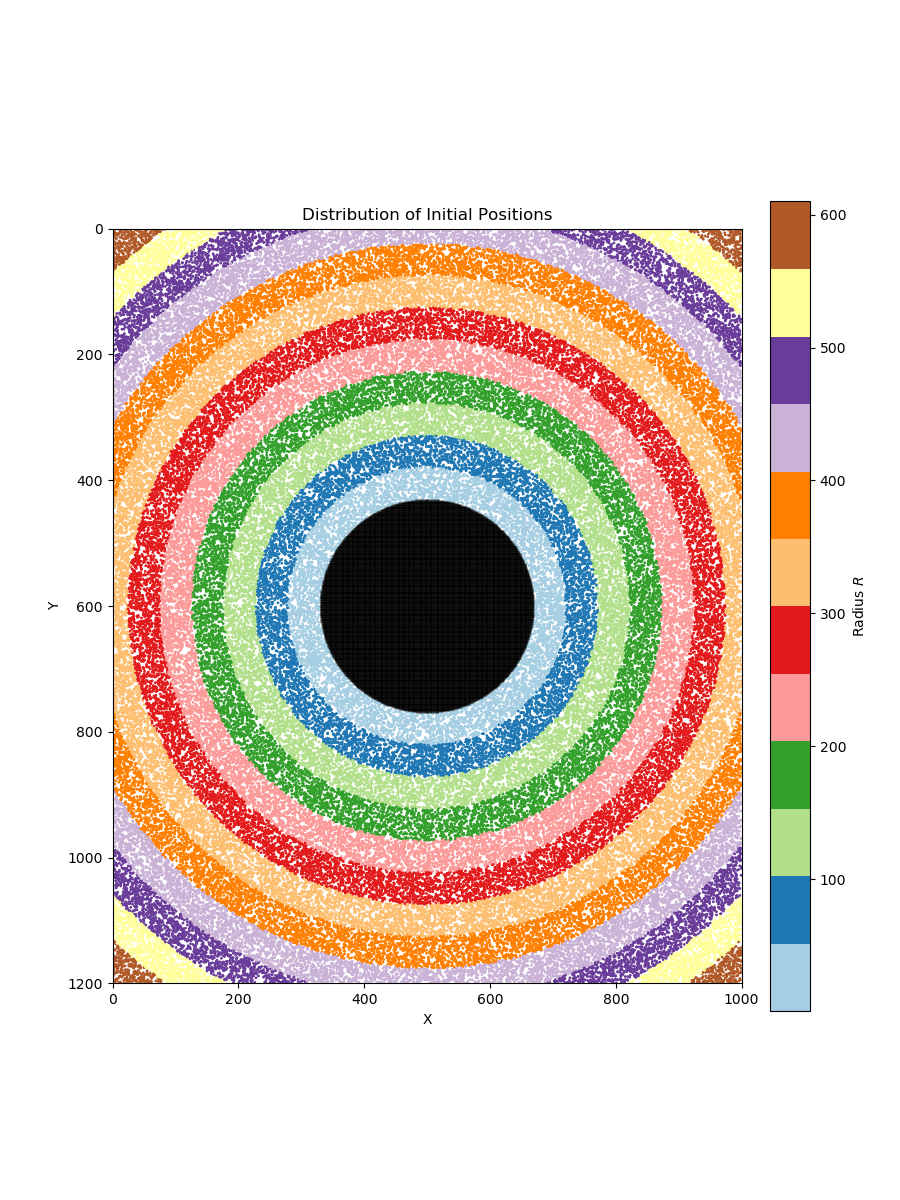
\includegraphics[width=\textwidth]{circle_initial_radius_color_initial_pos.png}
          \caption{}
          \label{fig:circle_radius_initial_pos}
        \end{subfigure}
        \caption{}
        \label{fig:radius_initial_pos}
     \end{figure}

     
     
   
   \subsubsection{Comparison of Survival Curves}


      \begin{figure}
        \centering      
        \begin{subfigure}[b]{0.45\textwidth}
          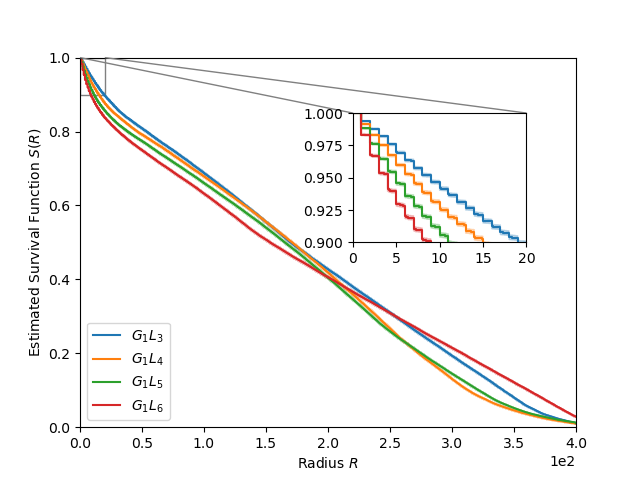
\includegraphics[width=\textwidth]{G_1_initial_radius_sf.png}
          \caption{}
          \label{fig:sf_g1_branch_radius}
        \end{subfigure}
        \hfill
        \begin{subfigure}[b]{0.45\textwidth}
          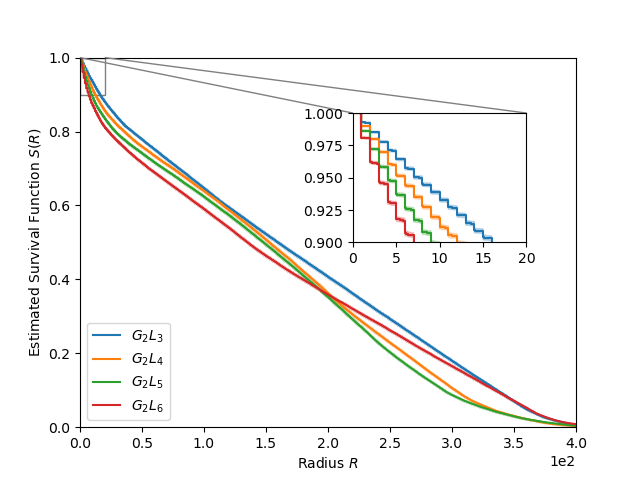
\includegraphics[width=\textwidth]{G_2_initial_radius_sf.png}
          \caption{}
          \label{fig:sf_g2_branch_radius}
        \end{subfigure}
        \caption{}
        \label{fig:sf_branch_radius}

      \end{figure}




      \begin{figure}
        \centering      
        \begin{subfigure}[b]{0.45\textwidth}
          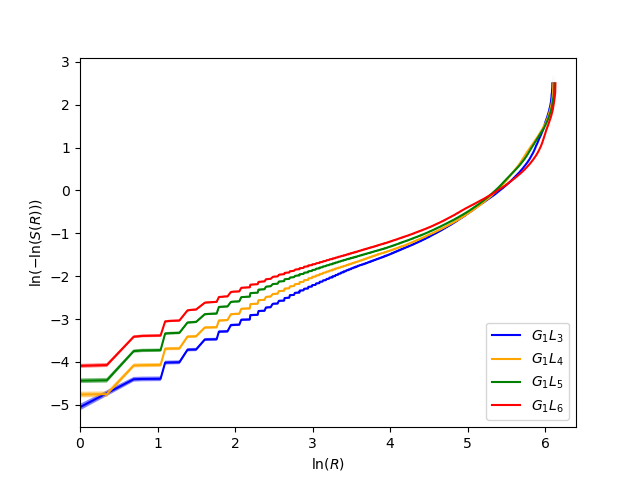
\includegraphics[width=\textwidth]{G_1_initial_radius_check_ph.png}
          \caption{}
          \label{fig:g1_branch_radius_check_ph}
        \end{subfigure}
        \hfill
        \begin{subfigure}[b]{0.45\textwidth}
          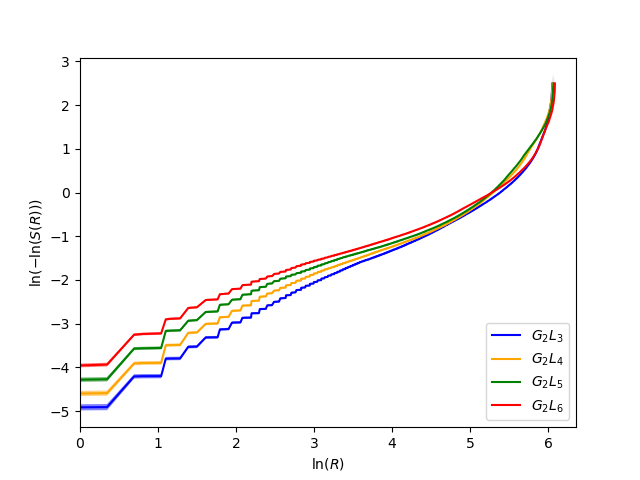
\includegraphics[width=\textwidth]{G_2_initial_radius_check_ph.png}
          \caption{}
          \label{fig:g2_branch_radius_check_ph}
        \end{subfigure}
        \caption{}
        \label{fig:branch_radius_check_ph}
      \end{figure}

      

      
      
      \begin{table}
        \centering
        \begin{tabular}{llrrrr}
          \toprule
                       &             &         &  p &    &     \\
          \cmidrule{3-6}
                       &             & Logrank & TW & GB & FH  \\
          \midrule
          $G_1$ $L_3$  & $G_1$ $L_4$  &  0.0 &  0.0 &  0.0 &  0.0     \\
                       & $G_1$ $L_5$  & 0.0 & 0.0 & 0.0 & 0.0    \\
                       & $G_1$ $L_6$  & 0.0 & 0.0 & 0.0 & 0.0      \\
          $G_1$ $L_4$  & $G_1$ $L_5$  & 0.1773 & 0.0 & 0.0 & 0.0      \\
                       & $G_1$ $L_6$  & 0.0 & 0.0 & 0.0 & 0.0       \\
          $G_1$ $L_5$   & $G_1$ $L_6$ & 0.0 &  0.0 & 0.0 & 0.0      \\
          \bottomrule
        \end{tabular}
        \label{tab:g1_ingroup_tests_radius}
        \caption{}
      \end{table}


      \begin{table}
        \centering
        \begin{tabular}{llrrrr}
          \toprule
                       &             &         &  p &    &     \\
          \cmidrule{3-6}
                       &             & Logrank & TW & GB & FH  \\
          \midrule
          $G_2$ $L_3$  & $G_2$ $L_4$  &  0.0 &  0.0 &  0.0 &  0.0     \\
                       & $G_2$ $L_5$  & 0.0 & 0.0 & 0.0 & 0.0    \\
                       & $G_2$ $L_6$  & 0.0 & 0.0 & 0.0 & 0.0      \\
          $G_2$ $L_4$  & $G_2$ $L_5$  & 0.0 & 0.0 & 0.0 & 0.0      \\
                       & $G_2$ $L_6$  & 0.0 & 0.0 & 0.0 & 0.0       \\
          $G_2$ $L_5$   & $G_2$ $L_6$ & 0.0 & 0.0 & 0.0253 & 0.0253      \\
          \bottomrule
        \end{tabular}
        \label{tab:g2_ingroup_tests_radius}
        \caption{}
      \end{table}


      \subsubsection{Distance Matrices}


      \subsubsection{Multidimenisonal Scaling}

















